    \section{Conclusion}

\subsection{Tesla}
\begin{frame}
\frametitle{Tesla}
\begin{center}
\begin{columns}
\begin{column}{330px}
{
    \begin{figure}[h!]
        \centering
        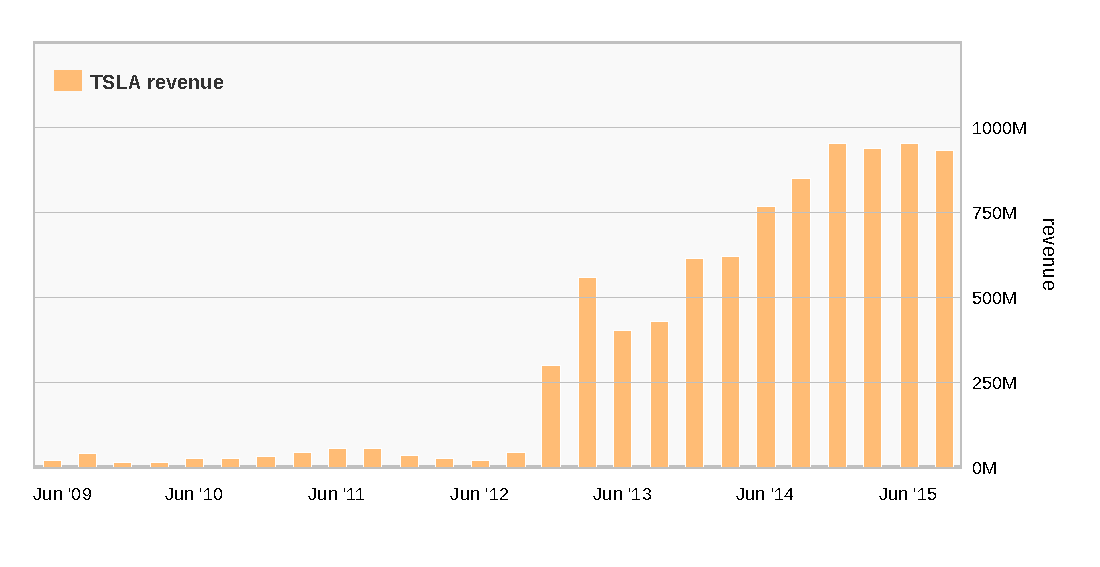
\includegraphics[width=310px]
            {images/TSLA-revenue-chart.eps}
        \vspace{-1em}
        \caption{Tesla Motors' revenue}
        \scriptsize{Source :
            \url{http://amigobulls.com}}
    \end{figure}
}
\end{column}
\end{columns}
\end{center}
\end{frame}


\begin{frame}
\begin{center}
\begin{columns}
\begin{column}{330px}
{
    \begin{figure}[h!]
        \centering
        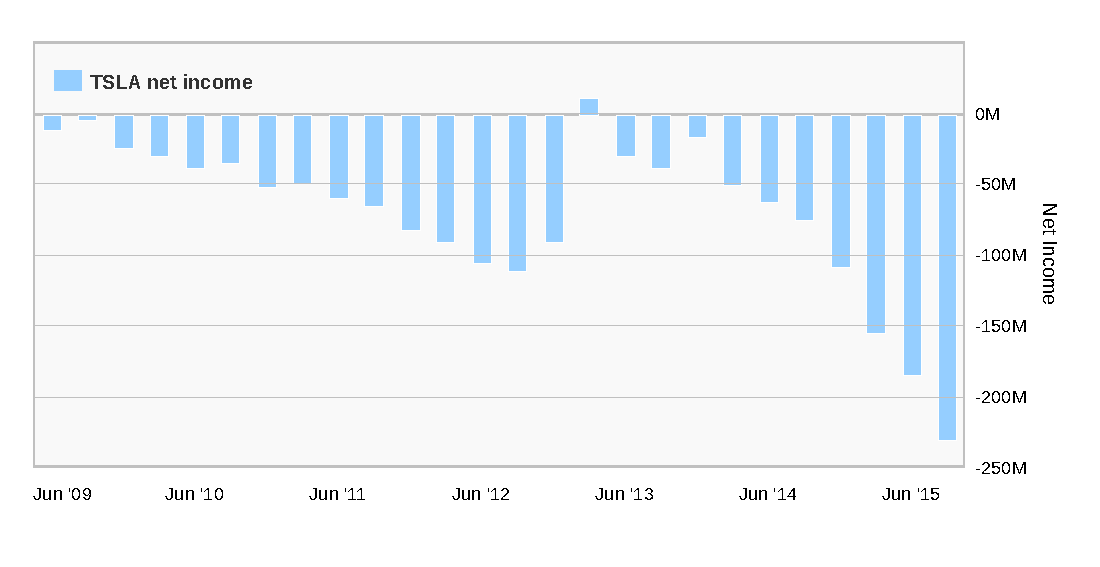
\includegraphics[width=310px]
            {images/TSLA-netincome-chart.eps}
        \vspace{-1em}
        \caption{Tesla Motors' net incomes}
        \scriptsize{Source :
            \url{http://amigobulls.com}}
    \end{figure}
}
\end{column}
\end{columns}
\end{center}
\end{frame}


\begin{frame}
\begin{center}
\begin{columns}
\begin{column}{330px}
{
    \begin{figure}[h!]
        \centering
        \includegraphics[width=200px]
            {images/tesla-vehicules-sales.jpg}
        \caption{Tesla Motors vehicules sales}
        \scriptsize{Source :
            \url{http://my.tesla.com}}
    \end{figure}
}
\end{column}
\end{columns}
\end{center}
\end{frame}


\begin{frame}
\end{frame}


\begin{frame}
\end{frame}


\begin{frame}
\frametitle{Gotcha!}
\begin{center}
\begin{columns}
\begin{column}{330px}
{
    \begin{figure}[h!]
        \centering
        \includegraphics[width=230px]
            {images/efficiency-thermal-motors.jpg}
        \vspace{-0.5em}
        \caption{Thermal motors efficiency}
        \vspace{-0.3em}
        \scriptsize{Source :
            \url{https://www.fueleconomy.gov}}
    \end{figure}
}
\end{column}
\end{columns}
\end{center}
\end{frame}


\begin{frame}
\begin{center}
\begin{columns}
\begin{column}{330px}
{
    \begin{figure}[h!]
        \centering
        \includegraphics[width=250px]
            {images/efficiency-electric-motors.jpg}
        \vspace{-0.5em}
        \caption{Electric motors efficiency}
        \vspace{-0.3em}
        \scriptsize{Source :
            \url{https://www.fueleconomy.gov}}
    \end{figure}
}
\end{column}
\end{columns}
\end{center}
\end{frame}


{
\logo{}
\begin{frame}
\begin{center}
\begin{columns}
\begin{column}{290px}
{
    \centering
    \vspace{-1em}
    \begin{table}
    \resizebox{\textwidth}{!}{%
        \begin{tabular}{|c|c|c|c|c|}
            \hline
            \multicolumn{5}{|p{40em}|}{\centering{\textbf{Comparison of tailpipe and upstream CO2
                emissions estimated in the MY 2014}}} \\
            \hline
            \multirow{2}{*}{\textbf{Vehicle}} & \multirow{2}{*}{\textbf{Tailpipe CO2 (g/mi)}} &
                \multicolumn{3}{|c|}{\textbf{Tailpipe + total upstream CO2 (g/mi)}} \\
            \cline{3-5}
            && \textbf{Low} & \textbf{Avg} & \textbf{High}\\
            \hline
            BMW i3 &0 &93 &175 &266\\
            \hline
            Honda Fit EV &0 &99 &185 &281\\
            \hline
            Nissan Leaf &0 &104 &194 &296\\
            \hline
            Mitsubishi i &0 &104 &195 &296\\
            \hline
            Ford Focus Electric &0 &111 &208 &316\\
            \hline
            \textbf{Tesla Model S (60 kWh)} &\textbf{0} &\textbf{122}
                &\textbf{229} &\textbf{348}\\
            \hline
            \textbf{Tesla Model S (85 kWh)} &\textbf{0} &\textbf{131}
                &\textbf{246} &\textbf{374}\\
            \hline
            Mercedes-Benz B-Class ED &0 &138 &259 &394\\
            \hline
            Toyota RAV4 EV &0 &153 &287 &436\\
            \hline
            \hline
            \multicolumn{1}{|p{10em}|}{\centering\textbf{{Average 2014 gasoline-powered
                car}}} &367 &400 &400 &400\\
            \hline
        \end{tabular}}
    \vspace{-0.5em}
    \caption{Electric motors efficiency}
    \vspace{-0.3em}
    \scriptsize{Source :
        \url{EPA}}
    \end{table}
}
\end{column}
\end{columns}
\end{center}
\end{frame}
}
